\documentclass[a4paper]{article}
\usepackage{amssymb}
\usepackage{amsmath}
\usepackage{multicol}
\usepackage{fancyhdr}
\usepackage{hyperref}
\usepackage{listings}
\usepackage{color}
\usepackage{tikz}
\usetikzlibrary{shapes,arrows}
\usepackage{pgfplots}
\usepackage{pgfplotstable}
\usepackage{graphicx}
\usepackage[]{mdframed}
\usepackage{algorithm2e}
\usepackage{svg}
\usepackage{enumitem}
\usepackage{refcount}
\usepackage{cleveref}
\usepackage{amssymb}
\usepackage{amsmath}
\usepackage{multicol}
\usepackage{fancyhdr}
\usepackage{hyperref}
\usepackage{listings}
\usepackage{color}
\usepackage{tikz}
\usetikzlibrary{shapes,arrows}
\usepackage{pgfplots}
\usepackage{pgfplotstable}
\usepackage{graphicx}
\usepackage[]{mdframed}
\usepackage{algorithm2e}
\usepackage{svg}
\usepackage{enumitem}
\usepackage{refcount}
\usepackage{cleveref}
\usepackage{cite}
\usepackage{bookmark}
% draw a frame around given text
\newcommand{\coderef}[1]{%
  \hyperref[#1]{Code \numberstringnum{\getrefnumber{#1}}}%
}
\newcommand{\argmin}{\operatornamewithlimits{argmin}}
\newcommand{\framedtext}[1]{%
\vspace{1em}%
\par%
\noindent\fbox{%
    \parbox{\dimexpr\linewidth-2\fboxsep-2\fboxrule}{#1}%
}%
\vspace{1em}%
}
\SetKwComment{Comment}{\# }{}
\newcommand{\norm}[1]{\left\lVert#1\right\rVert}



% HEADER/FOOTER DEFINITIONS
\fancyhf{}
\lhead{\pageHead}
\rhead{\rightmark}
\rfoot{Page \thepage}
\lfoot{\author}

% draw a frame around given text
\newcommand{\coderef}[1]{%
  \hyperref[#1]{Code \numberstringnum{\getrefnumber{#1}}}%
}
\newcommand{\argmin}{\operatornamewithlimits{argmin}}
\newcommand{\framedtext}[1]{%
\vspace{1em}%
\par%
\noindent\fbox{%
    \parbox{\dimexpr\linewidth-2\fboxsep-2\fboxrule}{#1}%
}%
\vspace{1em}%
}
\SetKwComment{Comment}{\# }{}

\begin{document}
\pagestyle{fancy}
\begin{multicols}{2}
\tableofcontents
\end{multicols}
\newpage

\section{Introduction}

\section{Theoretical Background (Math)}

\section{Nearest Centroid Classifier}
The first classification algorithm we will look into is the Nearest Centroid Classidfier.
It is a widely used algorithm for classification and is also one of the simplest ones to implement.
We will start by looking at the mathematical background of the algorithm and then implement it in Python.
This will help us to understand how to derive a classification algorithm from a mathematical model as well as the
limitations of machine learning models regarding assumptions it has towards the data.
Apart from this, the NNC is easy to interpret and easy to implement, which is a great starting point to get familiar with 
the Python programming language and the libraries we will use in this book.

\subsection{Motivation}
As in previous chapters mentioned, neuro scientists and other researchers used the brain as a blueprint for
designing theories. If we think about the neurology that is happening when
we want to do a categorization we understand on a neuronal level what happens to our brain.
Of course, only to some extend for some classes of cells. And we understand how humans
arrive at a certain category through psychological experiments. But we do not understand
how the brain is able to do this.
Between these two areas there is a huge gap. There is some research that tries to bridge this gap and ML could be a way to do this.
At last by providing some Prove of Concept (PoC) to those theories.
We will use a very simple psychological idea to explain the relation between the NCC and Linear Classifiers.
Linear Classification is on of the most frequently used techniques in Machine Learning. Even you do it, probably on a daily basis.
Now, we will bridge between the NCC and Linear Classifiers. But first we will try to understand the idea of classification through a psychological model.


\framedtext{
  \textbf{Imagine you are a Neuron.}

  You receive a non-linear filtered sensort input $\vec{x}$, e.g. a visual input from your eyes, a smell from your nose or a noice from your ears.

  \textit{How can we build abstract concepts from this information input?}

  In other words, \textit{how do humans categorize different stimuli?}
}\newline
For simplicity and to be able to visualize things we will imagine we only receive a 2 dimensional input.\\
First, we know all our data is $\vec{x} \in \mathbb{R}^2$. For example the bottom right triangle in Figure \ref{fig:prototypes_1} could be 
$\vec{x} = \begin{pmatrix}3\\2.5\end{pmatrix}$

\begin{figure}[h]
  \centering
  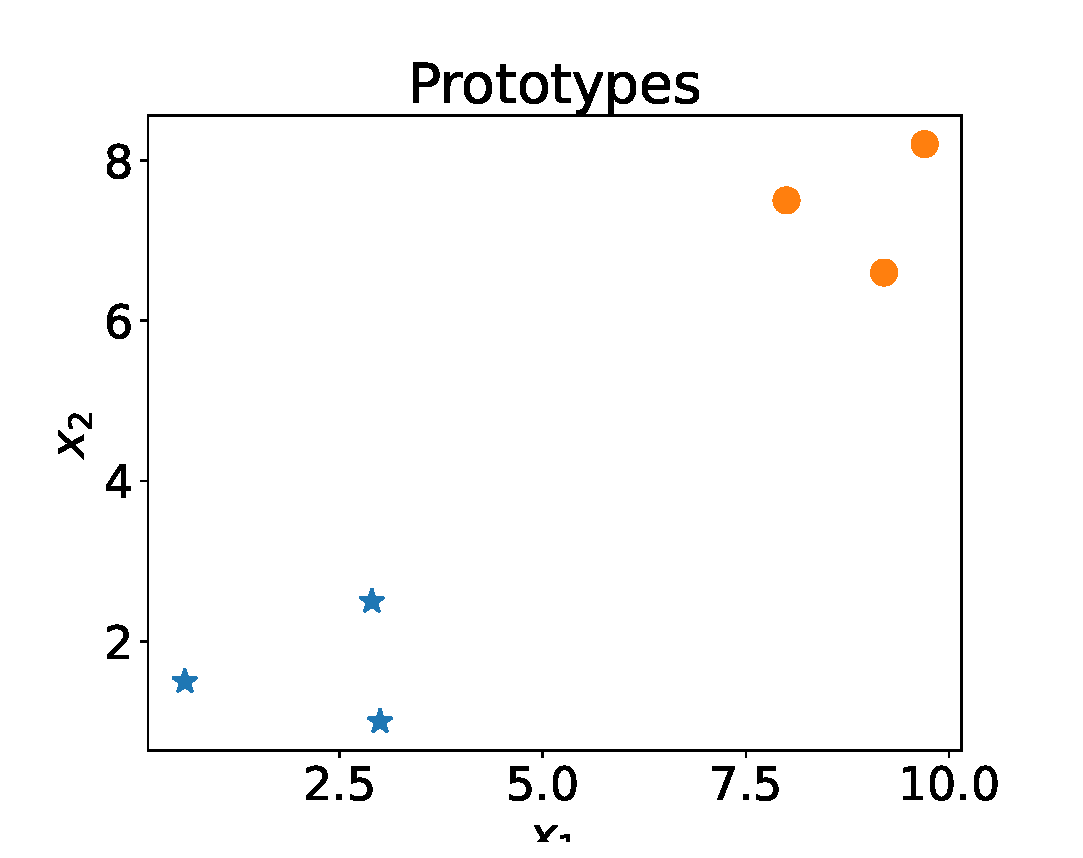
\includegraphics[width=.75\textwidth]{images/prototypes_0.eps}
  \caption{Prototypes of different categories}
  \label{fig:prototypes_0}
\end{figure}

We can also distinguish between two categories. For example, we could have a category of $\bigtriangleup$ and a category of $\bigcirc$.
Now, the question is: \textit{What do we do if we get a new data point?} For example $\vec{x}_{\times} = \begin{pmatrix}7.5\\4.0\end{pmatrix}$

\begin{figure}[h]
  \centering
  \includegraphics[width=.75\textwidth]{images/prototypes_1.eps}
  \caption{A new sample was added to the data set}
  \label{fig:prototypes_1}
\end{figure}

We need to find a mechanism of assigning a label to a new data point \textit{cross}.
For existing points we have this information already and we know which point belongs to which category. 
So how do we know which category the new point belongs to?

Psychiologists came up with the idea of designing so called \textit{prototypes} for each category.

This easiest solution for such prototype is calculating the \underline{mean} of all points in a category.
In this example we would compute the mean of all $\bigtriangleup$ $\mu_\bigtriangleup$ and the mean of all $\bigcirc$ $\mu_\bigcirc$.
\begin{figure}[h]
  \centering
  \includegraphics[width=.75\textwidth]{images/prototypes_2.eps}
  \caption{Mean values as prototypes for different categories}
  \label{fig:prototypes_2}
\end{figure}

The formula for the mean is:
\begin{equation}
  \mu = \frac{1}{N} \sum_{i=1}^{N} x_i
  \label{eq:mean}
\end{equation}
where $N$ is the number of samples and $x_i$ is the $i$-th sample.
For each of the categories this translates to
\begin{align}
  \mu_\bigtriangleup &= \frac{1}{N_\bigtriangleup} \sum_{i=1}^{N_\bigtriangleup} x_{\bigtriangleup, i} \\
  \mu_\bigcirc &= \frac{1}{N_\bigcirc} \sum_{i=1}^{N_\bigcirc} x_{\bigcirc, i}
\end{align}
A label for a new data point $\vec{x}_{\times}$ can now be assigned by calculating the distance to each of the prototypes $\mu_{\bigtriangleup}$ and $\mu_{\bigcirc}$ and assigning the label of the prototype with the smallest distance.

One method to compute these distances is the \textbf{Euclidean Distance}, which is defined as
\begin{equation}
  d(\vec{x}, \vec{y}) = \sqrt{\sum_{i=1}^{N} (x_i - y_i)^2} = \sqrt{(\vec{x} - \vec{y})^T (\vec{x} - \vec{y})}
\end{equation}
where $n$ is the number of dimensions of the vectors $\vec{x}$ and $\vec{y}$.
There are many more distance metrics, and throughout this book we will encounter a few of them, but for now we will stick to the Euclidean Distance.
After computing all distances they can be compared and the label of the prototype with the smallest distance can be assigned to the new data point.

\textbf{Congratulations!} You just implemented your first classification algorithm, the Nearest Centroid Classifier.
\subsection{Implementation}
In the following, we will look into different implementations of the NCC algorithm. And will look into two different approaches to compute the prototypes.
These two approaches can be used in most common Machine Learning algorithms.

\subsubsection{Inference}
The pseudo code to perform a classification (inference) using the NCC algirithm is very simple:
\begin{algorithm}
\LinesNumbered
\caption{\textbf{N}earest \textbf{C}entroid \textbf{C}lassifier Inference}\label{alg:ncc}
\KwData{$\vec{x}\in\mathbb{R}^D, \mu_k, k\in\{1,\dots,K\}$}
\KwResult{$k^*$}
\Comment*[h]{Compute nearest class centroid}\\
$k^* \gets \argmin_{k\in\{1,\dots,K\}} d(\vec{x}, \mu_k)$\;
\end{algorithm}

There are different ways to compute the centroids, here we used the means.
To compute the means we can use two different approaches, we call these approaches \textit{batch} and \textit{streaming}.
These terms might not 100\% match the common understanding of these terms, but we will use them to distinguish between the two approaches.

\textbf{Batched} refers to the fact that we compute the mean of all samples in a category at once. This approach requires
us to store all samples in memory and then compute the mean. This is the easier, but more expensive approach.

\textbf{Streaming} refers to the fact that we compute the mean of all samples in a category one by one. This approach does not require
us to store all samples in memory and is therefore more memory efficient. This approach is also called \textit{online} learning.

\subsubsection{Batched}
The batched approach is the easier one to implement. We simply store all samples in memory and then compute the mean.
\begin{algorithm}
\LinesNumbered
\caption{\textbf{NCC} Means (Batched)}\label{alg:ncc_batched}
\KwData{$\vec{x}\in\mathbb{R}^D, \mu_k, k\in\{1,\dots,K\}$}
\KwResult{means $\mu_k, k\in\{1\dots k\}$}
\Comment*[h]{Init means and counters for each class}\\
\Comment*[h]{Computation of class means}\\
\For{class $k$ in $K$}{
  $\mu_k \gets \frac{1}{N_k}\sum^{N_k}_{i=1}\vec{x_i}$\;
}
\end{algorithm}

\subsubsection{Streaming}
To derive the streaming approach we need to look at the mathematical definition of the batched version
\begin{equation}
  \mu_k = \frac{1}{N_k}\sum^{N_k}_{i=1}\vec{x_i}
\end{equation}
Imagine now, that we don't actually have the $N$-th data point yet.
We can rewrite the equation as
\begin{equation}
  \mu_k = \frac{1}{N_k}\sum^{N_k-1}_{i=1}\vec{x_i} + \frac{1}{N_k}\vec{x_N}
\end{equation}
We can see the factor $\frac{1}{N_k}$ is the same for all terms. This factor can be rewritten a bit differently
\begin{equation}
  \frac{1}{N_k} = \frac{1}{N_k-1} \cdot \frac{N_k-1}{N_k}
\end{equation}
Now we can rewrite the equation as
\begin{equation}
  \mu_k = \frac{1}{N_k}\sum^{N_k-1}_{i=1}\vec{x_i} + \frac{1}{N_k} \cdot \vec{x_N} = \frac{N_k - 1}{N_k}\frac{1}{N_k-1}\sum^{N_k-1}_{i=1}\vec{x_i} + \frac{1}{N_k} \cdot \vec{x_N}
\end{equation}
If we compare the middle term $\frac{1}{N_k}\sum^{N_k-1}_{i=1}\vec{x_i}$ with the original equation \eqref{eq:mean} we can see that it is just $\mu_{k-1}$.
\begin{equation}
  \Rightarrow \frac{N_k - 1}{N_k}\mu_{k-1} + \frac{1}{N_k} \cdot \vec{x_k}
  \label{eq:iterative-mean}
\end{equation}

This equation can be used to iteratively compute the mean of a category. We can start with $\mu_0 = \vec{0}$ and then compute the mean of each sample
by using the equation \eqref{eq:iterative-mean}.
\begin{algorithm}
\LinesNumbered
\caption{\textbf{NCC} Means (Streaming)}\label{alg:ncc_streaming}
\KwData{$\vec{x}\in\mathbb{R}^D$ labels $y_1, \dots, y_N\in\{1,\dots,K\}$}
\KwResult{means $\mu_k, k\in\{1\dots k\}$}
\Comment*[h]{Init means and counters for each class}\\
$\forall k:$ $\mu_k \gets \vec{0}, N_k = 0$\;
\For{Data point $i = 1,\dots,N$}{
  \Comment*[h]{Update means and counters}\\
  $k \gets y_i$\;
  $\mu_k \gets \frac{N_k}{N_k + 1}\mu_{k} + \frac{1}{N_k + 1} \cdot \vec{x_i}$\;
  $N_k \gets N_k + 1$\;
}
\end{algorithm}

\subsection{Limitations}
Once we implemented on of the two approaches we can use it to classify new data points. For the example above this might result in \textit{Decision Boundaries} as shown in Figure \ref{fig:ncc_db_0}.
\begin{figure}[h]
  \centering
  \includesvg[width=.75\textwidth]{images/NCC_DBs_0.svg}
  \caption{Decision Boundaries}
  \label{fig:ncc_db_0}
\end{figure}

The NCC is a very simple algorithm and therefore has some limitations.
\begin{itemize}
  \item The NCC is a linear classifier. This means it can only separate linearly separable data.
  \item The NCC is very sensitive to outliers. If there are outliers in the data set, the mean will be shifted towards the outlier.
  \item The NCC is very sensitive to the number of samples in each category. If there are more samples in one category than in another, the mean will be shifted towards the category with more samples.
\end{itemize}

Let us look at the first limitation, the NCC is a linear classifier. This means it can only separate linearly separable data, similar to the data in Figure \ref{fig:ncc_db_0}.
If we have data that is not linearly separable, the NCC will not be able to separate it. An example of such data is shown in Figure \ref{fig:ncc_db_1}.

\begin{figure}[h]
  \centering
  \includesvg[width=.75\textwidth]{images/NCC_DBs_1.svg}
  \caption{Non-linearly separable data}
  \label{fig:ncc_db_1}
\end{figure}
\newpage

\section{Nearest Neighbor Classifier}
\section{Hyperparameter Optimization}
\newpage
\section{Feature Extraction}
In this chapter we will talk about feature extraction, which is an essential part of any ML project/workflow.
We will introduce these by looking at a simple example and then look at some more advanced techniques.
After we covered most common approaches we will look into a very important concept, \underline{Machine Learning Pipelines}.

\subsection{Motivation}
Feature Extraction describes the transformations from any kind of data to vectors.
Until now, we always assumed to have a vector representation of our training data.
We used the notation of $\vec{x} \in \mathbb{R}^d$ to describe a $d$-dimensional data point.
To represent the full data set we used the convention $\vec{X} \in \mathbb{R}^{N \times d}$ 
a $N$-by-$d$ matrix, where each row represents a data point. This notation is commonly used among ML practitioners
and widely implemented in ML libraries. But it is not the only way to represent data. In fact, it is not even the most common way to represent data.
In this chapter we will look into different ways to represent data and how to transform data into a vector representation.

One of the most important things in solving a problem with an ML model is selecting correct features.
Most moder achievements in ML are not due to new algorithms, but due to better ways to extract features.
Thankfully, for most problems we do not need to use any fancy feature extraction techniques or bleeding edge research.
Classical, standard feature extraction techniques are sufficient to solve most problems in a satisfying manner.
In this chapter we will look into some of these techniques, but there are many more.
It is important to underline here, that often the best feature extractors are created by experts with domain knowledge.
Sometimes this expert can be you, but often it is not. In this case it is important to talk to the experts and understand the problem and challenges.
But for many problems and data types there are prebuild methods that we can apply without aquiring the domaing knowledge.
Imagine any work in the Natural Language Processing (NLP) field. It would be horribly bad if every ML practitioner would need to study linguistics prior
to working on an NLP problem.
Lastly, many of theses feature extraction techniques have to be optimized in order to achieve the best results possible. The easiest approach for this is trial and error.

In this chapter we look into four different types of data and different techniques how to extract features from them.

\subsection{Continuous Features}
Continuous features are the easiest to understand and to work with. They are also the most common type of data.
Continues data, is simply numerical data as real or integer values $x \in \mathbb{R}^d$. In many models continuous features are not required
to be transformed, because they can be used directly. But for some models it is benefitial to normalize continuous features.
For instance if we optimize our model with gradient descent (GD) or when we apply regularization to our model\footnote{Both of these ideas will be introduced in the future, but it is important to mention them here.}.

Given a feature $\vec{x} \in \mathbb{R}^d$ (analog for multivariant) there are several standard normalization options.
\subsubsection{Normalization: z-Score}
One of the normalization methods foro continuous features is the z-Score or standard scaling.
The z-Score is defined as
\begin{equation}
  z = \frac{x - \mu}{\sigma}
\end{equation}
where $\mu$ is the mean and $\sigma$ is the standard deviation of the feature.

In Python we can implement this as follows:
\begin{lstlisting}[language=Python, caption={z-Score in Python}, label={code:z-score}]
def z_score(X):
  return (X - X.mean(axis=0)) / X.std(axis=0)
\end{lstlisting}
Imagine the data set $\vec{X} \in \mathbb{R}^{N \times 1}$ ($N$ is the number of samples), then we can compute the mean of $\vec{X}$ through \lstinline{X.mean(axis=0)}.
Analogously this approach works for the multivariant case $\vec{X} \in \mathbb{R}^{N \times d}$.
The same applies for the standard deviation \lstinline{X.std(axis=0)}.
Putting everything together we get the z-Score for a data set $\vec{X}$ as implemented in \coderef{code:z-score}.
This method is also implemented in \lstinline{sklearn.preprocessing.StandardScaler}.
\subsubsection{Normalization: Min-Max-Scaling}
Another form of normalization is Min-Max-Scaling. 
The previous normalization method is great if your data is in the shape of a normal distribution.
If it isn't, you might as well chose Min-Max-Scaling, which ensures that the minimum values $\min(\vec{x})$ and maximum values $\max(\vec{x})$ of the scaled data are in a certain range, e.g. $[0, 1]$.
It does so by computing the min $\min(\vec{x})$ and max $\max(\vec{x})$ of the feature and then scaling the data as follows
\begin{equation}
  x_{scaled} = \frac{x - \min(\vec{x})}{\max(\vec{x}) - \min(\vec{x})}
\end{equation}
The resulting variable is in the range $[0, 1]$ or any other.
This method is also implemented in \lstinline{sklearn.preprocessing.MinMaxScaler}.
I leave the implementation as an exercise to the reader.
\subsection{Categorical Features}
As mentioned earlier continues features often don't need to be trasnformed. But categorical features most certainly need to be transformed.
Categorical features are variables $x \in C$ where $C$ can be any finite set of $N$ values without implicit ordering, e.g.
\begin{itemize}
  \item $C = \{red, green, blue\}$
  \item $C = \{dog, cat, mouse, horse\}$
  \item $C = \{1, 2, 6, 4, 5, 3\}$
  \item $C \in \{\text{User.id}\}$
\end{itemize}
The last example is a bit special, because it is not a finite set. But it is still a categorical feature, because it is not a continues feature.
The first three examples are called \textit{nominal} categorical features, because there is no implicit ordering.
To use these features in a ML model we need to transform them into a vector representation.
Here we will introduce the technique of \textit{One-Hot-Encoding} (OHE) to transform categorical features into a vector representation, but there are also
other techniques like for neural networks so called \textit{Embeddings}.
\subsubsection{One-Hot-Encoding}
We assume we have a fixed set of categorical values, e.g. $C = \{red, green, blue\}$. Then to generate the one-hot-encoding we first need to compute the cardinality of $C$.
The cardinality of a set is the number of elements in the set. In our example the cardinality of $C$ is $|C| = 3$. This means we need to transform each categorical value into a row-vector of length $|C|$.
For each categorical value we create a vector of length $|C|$ and set the value of the corresponding index to $1$ and all other values to $0$, so that
\begin{itemize}
  \item $red \rightarrow \begin{pmatrix}1 & 0 & 0\end{pmatrix}$
  \item $green \rightarrow \begin{pmatrix}0 & 1 & 0\end{pmatrix}$
  \item $blue \rightarrow \begin{pmatrix}0 & 0 & 1\end{pmatrix}$
\end{itemize}
By doing that categories can be easily represented as vectors.
This is also implemented in \lstinline{sklearn.preprocessing.OneHotEncoder}.
An example for using this approach are bag-of-words vectors, which we will look into in a second.

\subsubsection{One-hot-Encoding: Problems}
One of the main problems of OHE is that the cardinality of the categorical feature needs to be estimated upfront, i.e. prior to creation of the OHE vectors.
Therefore new items/categories can not be represented. Moreover, we lose the information on similarity between the categories, e.g. "light-blue" is as different as "green" to "blue".

\textbf{Note} In many situations we will face mixtures of continuous and categorical features. Usually we need to apply different extraction methods
to single features to put together a general feature representation of a sample.
\subsection{Text Features}
The next data type we will look into is text data. Again, we have several options here and especially lately this data type enjoys great popularity and research.
We will look at one approach more closely and shortly touch a few others.
The approach we will focus on is Bag-of-Words (BoW), a simple yet still very powerful technique that is very similar to the one-hot-encoding.
\subsubsection{Bag-of-Words Features}
To create BoW-Features we count the word occurrences in the given text. They are basically histograms of word occurrences.

\textbf{Example} Imagine we have the following text
\begin{quote}
  "The tokenizer splits the text into tokens."
\end{quote}
Then we can create a BoW-Feature vector as follows

\begin{table}[h]
  \centering
  \begin{tabular}{|l|ccccccc|}
    \hline
    \textbf{Word} & the & tokenizer & splits & text & into & tokens & . \\
    \hline
    \textbf{Count} & 2 & 1 & 1 & 1 & 1 & 1 & 1 \\
    \hline
  \end{tabular}
  \caption{BoW-Feature vector}
  \label{tab:bow}
\end{table}

How does this work?
\begin{enumerate}
  \item split the text into "tokens", e.g. words
  \item build one-hot-like vector for all found words
  \item count the occurrences of each word inside the text
\end{enumerate}
In the BoW approach $x$ is the vector of word occurrences. The name of an dimension is the word assigned to it.
$\vec{x} \in \mathbb{N}^d$ where $d$ is the number of unique words, the \underline{word vocabulary}, in the text.
$d$ needs to be determined prior to starting and can become quite big, which we will discuss in the following.
\subsubsection{Bag-of-Words: Problems}
BoW-Features only account for the word historgram and due to that most of the natural language structure is lost.
We lose for example the order of words, or context when processing multiple senteces at once.

Overall, BoW-Features are still very efficient and a reasonable approach.

\subsubsection{Bag-of-Words: Model with N-Grams}
To overcome the issue of losing language structure we can apply a different way of tokenizing our text document.
Before we used word-tokens, with N-Grams we use sequences of words, specifically sequences of $N$ words.
E.g. Bi-Grams constst of two words
\begin{table}[h]
  \centering
  \begin{tabular}{|l|ccccccc|}
    \hline
    \textbf{Word} & the tokenizer & tokenizer splits & splits the & the text & text into & into tokens & tokens . \\
    \hline
    \textbf{Count} & 1 & 1 & 1 & 1 & 1 & 1 & 1 \\
    \hline
  \end{tabular}
  \caption{BoW-Feature Bi-Gram vector}
  \label{tab:bow-bi-gram}
\end{table}
If we would consider every combination of words the dimensionality of this new vector $\vec{x}$ will also significantly change, because we represent sequences of words instead of single words now.
For the Bi-Gram example we get $x \in \mathbb{N}^{d^2}$ where $d$ is the number of unique Bi-Grams in the text.
An implementation of BoW-Features is available in sklearn's \lstinline{sklearn.feature_extraction.text.CountVectorizer}.

\subsubsection{Bag-of-Words: Character N-Grams}
We will briefly look into another approach to BoW-Features, which is using character N-Grams instead of word N-Grams.
This approach uses character sequences instead of word sequences. This approach is especially useful for languages with a rich morphology, e.g. German.
Another great application is for language independent models, e.g. for language detection.
Eseentially, we can select a tokenization method that fits our needs best, then transform these tokens into a BoW encoding.

\subsubsection{Term Frequency - Inverse Document Frequency (TF-IDF)}
One of the problems of using token occurrences is that natural language contains a lot of words that don't transfer information.
Frequently occurring words like "the" are often not meaningful and will be weighted down by the inverse document frequency.
Usually, we see a word-frequency distribution in the shape of the distribution shown in Figure \ref{fig:word-freq-dist}.

\begin{figure}[h]
  \centering
  \includegraphics[width=.95\textwidth]{images/word-distribution.png}
  \caption{Word frequency distribution from Moby Dick (https://www.gutenberg.org/ebooks/2701)}
  \label{fig:word-freq-dist}
\end{figure}
In order to downweight the frequencly occurring workds to be able to only select relevant words, we aplly the inverse
frequency
\begin{equation}
  \text{idf}(t, d) = \log \frac{|\text{Documents}|}{|\text{Documents containing } t|}
  \label{eq:TF-IDF}
\end{equation}
A model incorporating this idf metric is TFIDF which is essentially a BoW model with applied term frequency and idf.

In sklearn you can find it under \lstinline{sklearn.feature_extraction.text.TfidfVectorizer}.

\subsubsection{Stop-Words}
Another alternative to remove noice from our data are Stop-Words.
Instead of computing tf and idf, we have a set of predefined words to exclude from the document.
For most languages we can do that and prepare a set of words that won't change frequently.
From my experience they seem to work great, and I use them more often than TF-IDF.

\subsubsection{N-Grams are expensive}
We quickly jump back to the N-Gram tokens and discuss the dimensionality of our BoW vectors.

If we use unigrams ($N = 1$) the size of our vectors $\vec{x} \in \mathbb{R}^d$ is $d$ the size of our vocabulary.
The size of this is $v$ in the worst case. Libraries use so called sparse vectors to represent these
high dimensional data points, dense representations require too much memory by storing $0$ values.
When we increase $N$ to $N=2$ (Bi-Grams) this memory requirement grows by a factor of $d$. So the worst case
scenario increases to $d^2 \Rightarrow \vec{x} \in \mathbb{R}^{d^2}$.
But mostly we do not gain much from this, in terms of increasing the context that is encoded.
This applies annalogously to higher orders of N-Grams, e.g. $N=3$ (Tri-Grams) require $V^3$ dimensions and so on.
If we consider e.g. German as a language, and we know that the vocabulary for this language is somewhere in the realm of $d \approx 10^{12}$.
This will cause big memory issues, especially when using anything else but Uni-Grams.

Before neural networks and deep learning google provided big sets of N-Gram data for many languages, so no one must create them
themself. You can find up to $N=5$-Grams here: \url{http://storage.googleapis.com/books/ngrams/books/datasetsv2.html}.

\subsubsection{Hashed N-Grams}
Another optimization trick to reduce memory of N-Grams is using hash-maps.

For those who know about hash-maps, instead of representing words/tokens as vectors, each dimension corresponds to a hash bucket
using a hash function.
This can cause hash-collision, a problem where two or more values are hashed to the same hash-value. It appears when the number of hash-buckets
is lower than the number of $N$-Grams we want to store.
But because of the structure of natural language we rarely have multiple senteces containing the same words in different orders, the collision rate is low to insignificant.
I highly encourage the reader to try it out, if you run out of memory with regular vectorizers.

\subsection{Image Features}
We discussed until now continuous and categorical features, as well as text features.
To complete this we will briefly look at methods to extract features from images.
Due to the complexity of these methods we will only motivate them, because thoroughly understanding them would go beyond the scope of this book.
Most of them are very easy to use, but hard to understand.

\subsubsection{Classical Computer Vision}
Before 2012 (ImageNet Moment) researches used classic CV methods to extract features from images.
Mostly Furrier Decomposition was applied, this measures spacial frequencies of patches of the image.
The resulting frequency strength of each patch is then used as a feature.
These spacial frequencies are gradients in the image. High spacial frequencies are edges,
and the phase of the frequency is its orientation.
These kind of features are computed in the \underline{Histogram of Oriented Gradients/Edges} (HOG) feature extractor, as showcased in 
Figure \ref{fig:hog}.

\begin{figure}[h]
  \centering
  \includegraphics[width=.95\textwidth]{images/hog.png}
  \caption{HOG feature extraction}
  \label{fig:hog}
\end{figure}

HOG suits very well for object detection, because it is very robust to changes in illumination and other factors.
For this reason it is widely used in e.g. self-driving cars for pedestrian recognition.
They work good if we only want to encode a shape, e.g. a pedestrian, but not for more complex tasks like face recognition.
In skimage you can find the HOG extractor in \lstinline{skimage.feature.hog}.

\subsubsection{Convolutional Neural Networks}
Another more modern way of dealing with images is using Convolutional Neural Networks (CNNs).
They are state-of-the-art (SOTA) for image classification and object detection.
We don't have much time to look detaied into them, but the key takeaway here is:

We won't train these models from scratch. We will apply pretrained models, because we won't
be able to achieve same performance with models we would train ourselves.
And we don't want to spend so much time and money on training these models.
Thankfully, we don't need to because there are many pretrained models publicly available.
These models are trained foro a long time on very large datasets, e.g. ImageNet\cite{deng2009imagenet}, for us!
All we have to do is to download these models and run them as feature extractors.
You can read more about CNNs in my these \cite{PhilippZettl:2022}.

\section{Machine Learning Pipelines}
Recall the pipeline diagram from the first chapter.

\begin{figure}[h]
  \centering
  \begin{tikzpicture}
    \node[draw, rectangle] (data) at (0, 0) {Data};
    \node[draw, rectangle] (features) at (2.5, 0) {\begin{tabular}{c}Feature\\Extraction\end{tabular}};
    \node[draw, rectangle, minimum height=2cm, minimum width=6.25cm] () at (4.25, 0) {};
    \node[draw, rectangle] (model) at (6, 0) {\begin{tabular}{c}ML Model\\$f(x)$\end{tabular}};
    \node[draw, rectangle] (prediction) at (9, 0) {Prediction};
    \draw[->] (data) -- (features);
    \draw[->] (features) -- (model);
    \draw[->] (model) -- (prediction);
  \end{tikzpicture}
  \caption{Machine Learning Pipeline}
  \label{fig:ml-pipeline}
\end{figure}
Up until now we always assumed to have a vector representation $\vec{x}\in\mathbb{R}^d$ of our data.
Starting from now, our data might be in any other format, like text or images.

To build a system that gets a certain format of input, transform this input into $d$ dimensional vectors and feeds them into our model.
We will now look at how to program such an ML-Pipeline
\subsection{Motivation}
In the previous chapters we looked into different feature extraction techniques.
We also looked in previous chapters into different ML models and how to train them.
Now, we will look into how to combine these two concepts into a single pipeline.

One way how to implement this is to manually write code that executes all steps of the pipeline sequentially.
But this would be quite static and not very flexible. We would need to rewrite the code for every new data set or whenever
we want to change a part of the pipeline.

A better way to implement this is to use a so called \textit{Pipeline} object. This object is a wrapper around all steps of the pipeline.
The most popular API-Interface for this is implemented by the guys from scikit-learn \cite{scikit-learn}.

We will look into the implementation of such a pipeline in the following because it will allow to combine
own implementations with implementations inside scikit-learn. This is especially useful because scikit-learn
delivers plenty of tools, feature extraction algorithms and model architectures.

I personally work a lot with scikit-learn and I highly recommend it to anyone who wants to get started with ML as well assigned
encourage everyone to contribute to the project.

\subsection{Estimators}


\section{Metrics}
\section{Model Evaluation}
\section{Perceptron}
\section{Decision Trees}
\section{Regression}
\section{Principal Component Analysis (PCA)}
\section{Clustering}
\section{Neural Networks}

\bibliographystyle{ieeetr}
\bibliography{refs} % Entries are in the refs.bib file
\end{document}
